\documentclass{article}
\usepackage{tikz}

\begin{document}

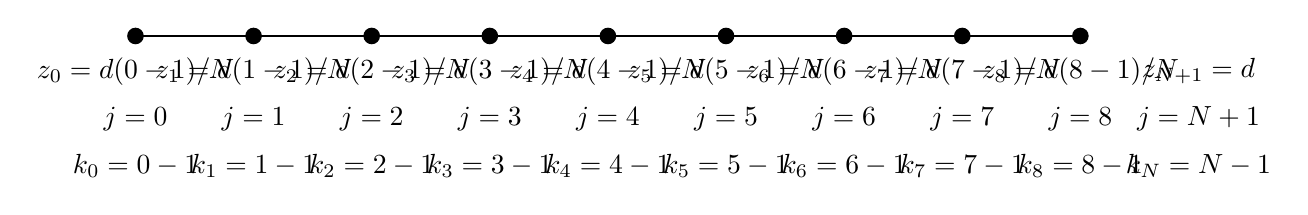
\begin{tikzpicture}[scale=1.5]
    % Draw the horizontal line
    \draw (0,0) -- (8,0);
    
    % Place the nodes with their labels
    \foreach \x in {0,1,...,8} {
        \fill (\x,0) circle (2pt);
        \node at (\x,-0.3) {$z_{\x} = d(\x-1)/N$};
        \node at (\x,-0.7) {$j=\x$};
        \node at (\x,-1.1) {$k_{\x}= \x - 1$};
    }
    
    % Add the special case for the last node
    \node at (9,-0.3) {$z_{N+1} = d$};
    \node at (9,-0.7) {$j=N+1$};
    \node at (9,-1.1) {$k_{N}= N-1$};
\end{tikzpicture}

\end{document}